\chapter{Рекуррентные модели}
\label{chap:rnns}

\begin{supportbox}{Об этой главе}
Трансформерные модели очень эффективны при обработке последовательностей, но их сдерживает квадратичная сложность по длине последовательности. Одна из возможностей — заменить их рекуррентными слоями, имеющими только постоянное время для обработки каждого элемента последовательности, независимо от ее длины. В этой заключительной главе мы предоставляем широкий обзор за счет точности — см. \cite{tiezzi2024state} для недавнего обзора.
\end{supportbox}

\section{Линеаризованные модели внимания}
\subsection{Замена скалярного произведения}
\label{sec:linearized_transformer_model}

Чтобы дать некоторое представление о том, почему рекуррентные нейронные сети (РНС) могут быть полезны, мы начнем с обобщения слоя внимания (называемого \textbf{линеаризованным слоем внимания} \cite{katharopoulos2020transformers}), который можно записать в рекуррентной форме. Мы начнем с переписывания слоя SA в абстрактной форме с общей скалярной функцией внимания $\alpha(\cdot, \cdot)$ вместо скалярного произведения:
%
\begin{equation}
\mathbf{h}_i=\frac{\sum_{j=1}^n\alpha\left(\mathbf{q}_i, \mathbf{k}_j\right)\mathbf{v}_j}{\sum_{j=1}^n \alpha\left(\mathbf{q}_i, \mathbf{k}_j\right)}
\label{eq:generalized_attention}
\end{equation}
%
где для стандартного SA, $\alpha(\mathbf{x}, \mathbf{y})=\exp(\mathbf{x}^\top\mathbf{y})$. Если элементы последовательности должны обрабатываться по порядку (как при авторегрессионной генерации), \eqref{eq:generalized_attention} неудобно, потому что его стоимость растет квадратично с длиной последовательности. Даже если используется кэш KV, память все равно растет линейно. Для сравнения, свёрточный слой имеет фиксированную временную и пространственную стоимость для каждого обрабатываемого элемента, но информация теряется, если токен находится за пределами рецептивного поля. Вместо этого мы хотели бы иметь механизм для сжатия всей информации последовательности в вход фиксированного размера (который мы будем называть тензором \textbf{памяти} или \textbf{состояния}), чтобы стоимость запуска модели на нашем текущем входном токене плюс память была постоянной. Мы называем модели такой формы \textbf{рекуррентными}.

Для начала отметим, что любая неотрицательная $\alpha$ является допустимой функцией сходства. В машинном обучении это требование эквивалентно тому, что $\alpha$ является так называемой \textbf{ядерной функцией} \cite{hofmann2008kernel}. Многие такие ядерные функции можно записать как обобщенное скалярное произведение:
%
\begin{equation}
\alpha(\mathbf{x}, \mathbf{y})=\phi(\mathbf{x})^\top \phi(\mathbf{y})
\label{eq:kernel}
\end{equation}
%
для некоторой функции $\phi: \mathbb{R}^c \rightarrow \mathbb{R}^e$, которая выполняет расширение признаков. 

\begin{supportbox}{Ядерные функции}
В качестве примера, \textbf{полиномиальная ядерная функция} $\alpha(\mathbf{x}, \mathbf{y})=(1 + \mathbf{x}^\top\mathbf{y})^d$ может быть переписана как \eqref{eq:kernel}, если $\phi(\bullet)$ явно вычисляет все полиномы своего входа до порядка $d$ \cite{hofmann2008kernel}. Некоторые ядерные функции соответствуют бесконечномерным расширениям (например, гауссово ядро), и в этом случае (2) все еще можно восстановить в терминах приближенного расширения ядра, например, работая со случайными признаками Фурье \cite{scardapane2017randomness}.
\end{supportbox}
%
На основе \eqref{eq:kernel} мы можем переписать \eqref{eq:generalized_attention} как:
%
$$
\mathbf{h}_i=\frac{\sum_{j=1}^n \phi(\mathbf{q}_i)^\top\phi(\mathbf{k}_j)\mathbf{v}_j^\top}{\sum_{j=1}^n \phi(\mathbf{q}_i)^\top\phi(\mathbf{k}_j)}
$$
%
где мы добавили операцию транспонирования к $\mathbf{v}_j$, чтобы соответствовать размерностям. Поскольку $\phi(\mathbf{q}_i)$ не зависит от $j$, мы можем вынести его за знак суммы, чтобы получить:
%
\begin{equation}
\mathbf{h}_i=\frac{{\color{drawred}\phi(\mathbf{q}_i)^\top}\sum_{j=1}^n \phi(\mathbf{k}_j)\mathbf{v}_j^\top}{{\color{drawred}\phi(\mathbf{q}_i)^\top}\sum_{j=1}^n \phi(\mathbf{k}_j)}
\label{eq:linearized_attention}
\end{equation}
%
Это называется \textbf{линеаризованной моделью внимания} \cite{katharopoulos2020transformers}. Вычисление \eqref{eq:linearized_attention} для всех токенов имеет сложность $\mathcal{O}(n(e^2 + ev))$, что является линейным по длине последовательности и выгодно, когда $n <e^2$. $\phi$ можно выбирать свободно, например, в \cite{katharopoulos2020transformers} они рассматривают квадратичное расширение признаков или даже более простое $\phi(\mathbf{x})=\text{ELU}(\mathbf{x})+1$ для коротких последовательностей.

\subsection{Рекуррентная формулировка}

Теперь мы перепишем линеаризованную модель внимания в рекуррентной форме, рассмотрев, что происходит для причинного варианта слоя. Во-первых, мы изменим \eqref{eq:linearized_attention}, ограничив сумму только прошлыми входными элементами, чтобы сделать ее причинной:

\begin{equation}
\mathbf{h}_i=\frac{\phi(\mathbf{q}_i)^\top\eqnmarkbox[drawred]{node}{\sum_{j=1}^{\color{drawred}i} \phi(\mathbf{k}_j)\mathbf{v}_j^\top}}{\phi(\mathbf{q}_i)^\top\eqnmarkbox[drawgreen]{node2}{\sum_{j=1}^{\color{drawred}i} \phi(\mathbf{k}_j)}}
\label{eq:atf}
\end{equation}
\annotate[yshift=1em]{above,right}{node}{Память внимания $\mathbf{S}_i$}
\annotate[yshift=-1em]{below,right}{node2}{Память нормализатора $\mathbf{z}_i$}

\vspace{1em}
Это наш первый пример \textbf{рекуррентного слоя}. Чтобы понять название, мы отмечаем, что память внимания и нормализатора можно записать рекурсивно как:
%
\begin{gather}
\mathbf{S}_i =\mathbf{S}_{i-1} + \phi(\mathbf{k}_i)\mathbf{v}_i^\top \label{eq:atf_recurrent_1} \\
\mathbf{z}_i = \mathbf{z}_{i-1}+\phi(\mathbf{k}_i) \label{eq:atf_recurrent_2}
\end{gather}
%
где базовый случай рекурсии задается их инициализацией:
%
\begin{gather}
\mathbf{S}_0=\mathbf{0} \\ \mathbf{z}_0=\mathbf{0}
\label{eq:atf_recurrent_init}
\end{gather}
%
Выход тогда задается как:
%
\begin{gather}
\mathbf{h}_i=\frac{\phi(\mathbf{q}_i)^\top\mathbf{S}_i}{\phi(\mathbf{q}_i)^\top\mathbf{z}_i} \label{eq:atf_recurrent_3}
\end{gather}
%
Уравнения \eqref{eq:atf_recurrent_1}-\eqref{eq:atf_recurrent_3} особенно интересны для авторегрессионного сценария: для каждого нового генерируемого токена мы обновляем два состояния памяти (уравнения \eqref{eq:atf_recurrent_1} и \eqref{eq:atf_recurrent_2}) и используем эти обновленные состояния для вычисления выхода для $i$-го элемента. Важно, что общие вычисления для генерации нового токена постоянны, и стоимость памяти также фиксирована, поскольку предыдущие памяти $\mathbf{S}_{i-1}$ и $\mathbf{z}_{i-1}$ можно отбросить. Мы можем чередовать две формулировки слоя: мы можем использовать векторизованный вариант для обучения (для эффективной реализации на GPU) и рекуррентную формулировку для вывода. 

\section{Классические рекуррентные слои}
\subsection{Общая формулировка}

\begin{SCfigure}
    \centering
    \hspace{2em}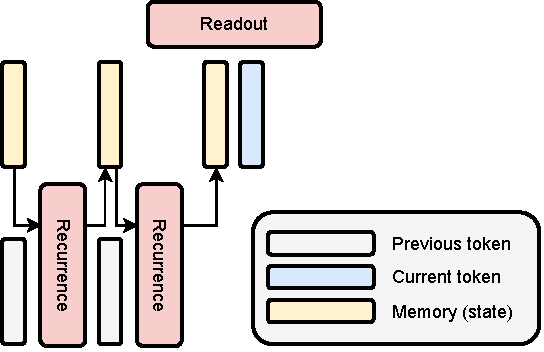
\includegraphics[width=0.5\textwidth]{images/recurrence}
    \caption{Обзор рекуррентного слоя: прошлые токены показаны серым, текущий входной токен — синим, состояние памяти — желтым.}
    \label{fig:recurrence}
\end{SCfigure}

Теперь давайте абстрагируемся от ключевых компонентов рекуррентного слоя, используя предыдущий раздел в качестве ориентира. Во-первых, нам нужно \textbf{состояние} фиксированного размера, которое используется для сжатия всей полезной информации до $i$-го элемента последовательности. Мы обозначаем его в общем виде как $\mathbf{s}_i$, и без потери общности мы будем предполагать, что это один вектор. Во-вторых, нам нужна \textbf{функция перехода} (рекурренция), которая обновляет вектор состояния на основе предыдущего значения и значения текущего токена, которую мы обозначаем как $f(\mathbf{s}_{i-1}, \mathbf{x}_i)$. В-третьих, нам нужна то, что мы называем \textbf{функцией считывания}, которая предоставляет выход для $i$-го элемента последовательности. Мы обозначаем ее как $g(\mathbf{s}_i, \mathbf{x}_i)$. См. также Рисунок \ref{fig:recurrence} для визуализации. 

\begin{definition}[Рекуррентный слой] \addbottle
%
Для последовательности токенов $\mathbf{x}_1, \mathbf{x}_2, \ldots$, общий рекуррентный слой можно записать как: 
%
\begin{gather}
\mathbf{s}_i = f(\mathbf{s}_{i-1},\mathbf{x}_i) \label{eq:recurrent_layer_state_update} \\
\mathbf{h}_i = g(\mathbf{s}_i, \mathbf{x}_i) \label{eq:recurrent_layer_readout}
\end{gather}
%
где \textbf{вектор состояния} $\mathbf{s}_i \sim (e)$ по соглашению инициализируется нулем, $\mathbf{s}_0 = \mathbf{0}$. Размер вектора состояния, $e$, и размер выходного вектора $\mathbf{h}_i \sim (o)$ являются гиперпараметрами. Мы называем $f$ функцией \textbf{перехода состояния}, а $g$ — функцией \textbf{считывания}.
%
\end{definition}

%
В этом формате рекуррентный слой представляет собой дискретную по времени, управляемую входом динамическую систему, и по определению является причинным слоем. В инженерии управления это также известно как \textbf{модель в пространстве состояний}. Для задач, в которых причинность не нужна, также можно определить \textbf{двунаправленные слои} \cite{schuster1997bidirectional}. В двунаправленном слое мы инициализируем два рекуррентных слоя (с отдельными параметрами), один из которых обрабатывает последовательность слева направо, а второй — справа налево. Их выходные состояния затем объединяются для получения окончательного выхода. 

Рекуррентные нейронные сети (РНС) можно строить, объединяя несколько рекуррентных слоев на обновленной последовательности $\mathbf{h}_1, \mathbf{h}_2, \ldots, \mathbf{h}_n$ \cite{pascanu2013construct}. Интересно, что рекуррентный слой не имеет требований к длине последовательности, которая (в принципе) может быть неограниченной. По этой причине можно показать, что РНС с неограниченной точностью или растущими архитектурами являются Тьюринг-полными \cite{chung2021turing}.

\begin{supportbox}{Неявные слои}
%
Что произойдет, если мы применим рекуррентный слой к \textit{одному} токену $\mathbf{x}$?
%
\begin{equation}
\mathbf{s}_i = f(\mathbf{s}_{i-1}, \mathbf{x})
\label{eq:recurrent_layer_single_token}
\end{equation}
%
Если мы запустим переход состояния несколько раз, начиная с известной инициализации $\mathbf{s}_0$, это будет похоже на модель с несколькими слоями (по одному на переход), разделяющими одни и те же параметры. Предположим, мы запускаем \eqref{eq:recurrent_layer_single_token} \textit{бесконечное} количество раз. Если динамическая система имеет стабильный аттрактор, выход будет определяться уравнением неподвижной точки:
%
\begin{equation}
\mathbf{s} = f(\mathbf{s}, \mathbf{x})
\label{eq:fixed_point_layer}
\end{equation}
%
Если мы возьмем \eqref{eq:fixed_point_layer} в качестве определения слоя, мы получим то, что называется \textbf{неявным слоем} \cite{bai2019deep}. Реализацию неявных слоев можно сделать возможной, используя быстрые решатели для уравнения неподвижной точки и вычисляя обратный проход с использованием \textbf{теоремы о неявной функции} \cite{bai2019deep}. Неявные графовые слои также можно определить, запуская каждую операцию диффузии до стабильного состояния \cite{gori2005new,scarselli2008graph}. 
%
\end{supportbox}

\vspace{-0.5em}
\subsection{«Ванильные» рекуррентные слои} \addclock

Исторически рекуррентные слои инстанцировались путем рассмотрения двух полносвязных слоев в качестве функций перехода и считывания:
%
\begin{gather}
f(\mathbf{s}_{i-1},\mathbf{x}_i)= \phi(\mathbf{A}\mathbf{s}_{i-1}+\mathbf{B}\mathbf{x}_i)\\g(\mathbf{s}_i,\mathbf{x}_i)=\mathbf{C}\mathbf{s}_i+\mathbf{D}\mathbf{x}_i
\end{gather}
%
где, как всегда, мы игнорируем смещения для простоты, и у нас есть четыре обучаемые матрицы $\mathbf{A} \sim (e,e)$, $\mathbf{B} \sim (e,c)$, $\mathbf{C} \sim (o,e)$ и $\mathbf{D} \sim (o,c)$, где $c$ — размерность входа (размер каждого токена). Слой в этой форме иногда называют в общем «\textit{рекуррентным слоем}», «\textit{ванильным рекуррентным слоем}» или рекуррентным слоем \textbf{Элмана}. Когда две матрицы $\mathbf{A}$ и $\mathbf{B}$ остаются необученными, и у нас есть только один слой, эти модели называются \textbf{сетями эхо-состояний} (ESN) или \textbf{резервуарными компьютерами} \cite{lukovsevivcius2009reservoir}. ESN могут быть мощной базовой линией для прогнозирования временных рядов, особенно когда необученные матрицы (резервуар) инициализируются должным образом \cite{gauthier2021next}.

Несмотря на их историческое значение, слои такой формы чрезвычайно неэффективны (и трудны) для обучения. Чтобы убедиться в этом, обратите внимание, что по своей конструкции вычисления по элементам последовательности не могут быть эффективно распараллелены, как показано в Листинге \ref{code:recurrence}. Следовательно, нам нужно прибегать к итерационным (for-циклам) реализациям, и даже высокоспециализированные реализации CUDA\footnote{\url{https://docs.nvidia.com/deeplearning/performance/dl-performance-recurrent/index.html}} медленнее, чем большинство альтернативных слоев последовательностей. 

\begin{mypy}{Ванильная рекурренция в PyTorch. Невозможно распараллелить for-цикл с помощью линейной алгебры из-за зависимостей в рекурренции. В PyTorch обновление состояния называется \textbf{рекуррентной ячейкой}, в то время как рекуррентные слои, такие как {\footnotesize\mintinline{python}{torch.nn.RNN}}, оборачивают ячейку и выполняют полный for-цикл.}{code:recurrence}
# Входной тензор
x = torch.randn(batch_size, sequence_length, features)

# Тензор состояния
s = torch.zeros(batch_size, state_size)

# Обновление состояния
state_update = nn.RNNCell(features, state_size)
for i in range(x.shape[1]):
  s = state_update(x[:, i, :], s)
\end{mypy}

Другая проблема связана с градиентами, участвующими в вычислениях слоя. Рассмотрим упрощенный случай, имеющий только функцию перехода. Мы можем развернуть полное вычисление как:
%$
\begin{gather*}\mathbf{s}_1=f(\mathbf{s}_0,\mathbf{x}_1) \\ \mathbf{s}_2=f(\mathbf{s}_1,\mathbf{x}_2) \\ \vdots \\ \mathbf{s}_n=f(\mathbf{s}_{n-1},\mathbf{x}_n)\end{gather*}
%
Это похоже на модель с $n$ слоями, за исключением того, что параметры разделяются (одинаковы) между слоями. Ниже мы сосредоточимся на величине $\partial_{\mathbf{A}} \mathbf{s}_n$ (весовой Якобиан по отношению к $\mathbf{A}$), но аналогичные соображения применимы ко всем градиентам. Давайте определим следующее кумулятивное произведение:
%
\begin{equation}\widetilde{\mathbf{s}}_i = \prod_{j={i+1}}^{n}\partial_{\mathbf{s}_{j-1} }f(\mathbf{s}_{j-1},\mathbf{x}_j)\end{equation}
%
Это представляет собой градиент функции перехода от конца последовательности назад к элементу $i$, как показано на Рисунке \ref{fig:recurrence_backward}. Из-за разделения весов искомый градиент имеет отдельный член для каждого элемента в последовательности, который включает эти кумулятивные произведения:
%
\begin{equation} 
\partial_{\mathbf{A}} \mathbf{s}_n = \eqnmarkbox[drawred]{node}{\partial_{\mathbf{A}} f(\mathbf{s}_{n-1}, \mathbf{x}_n)} + \sum_{i=1}^{n-1}  \eqnmarkbox[drawgreen]{node2}{\widetilde{\mathbf{s}}_i \bigl[ \partial_{\mathbf{A}} f(\mathbf{s}_{i-1}, \mathbf{x}_i)\bigr]}
\label{eq:backpropagation_through_time}
\end{equation}
\annotate[yshift=-1em]{below,left}{node}{Градиент от элемента $n$}
\annotate[yshift=-1em]{below,right}{node2}{Градиент от элемента $i$}

\begin{SCfigure}
    \centering
    \hspace{2em}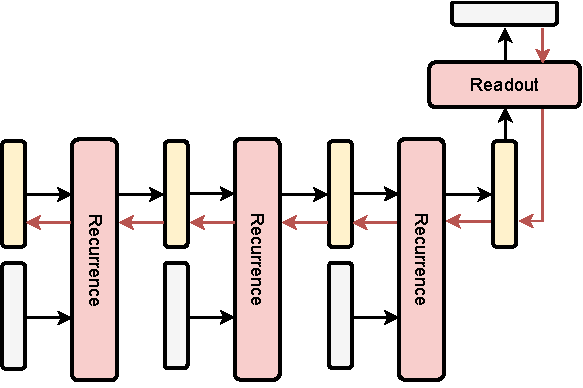
\includegraphics[width=0.5\textwidth]{images/recurrence-Pagina-2}
    \caption{Обратный проход для рекуррентного слоя: сопряженные значения должны распространяться через все шаги перехода. Каждое состояние затем вносит один член в полный градиент параметров.}
    \label{fig:recurrence_backward}
\end{SCfigure}

Первый член соответствует «стандартному» весовому Якобиану, описывающему влияние $\mathbf{A}$ на последний элемент последовательности. Члены в сумме — это дополнительные вклады, по одному для каждого элемента последовательности, которые взвешиваются цепным входным Якобианом, вычисленным по самой последовательности. 

Записанное в этой форме, автоматическое дифференцирование в обратном режиме также называется \textbf{обратным распространением ошибки во времени} (BPTT) и может быть сильным источником нестабильности или проблем с градиентами во время градиентного спуска. Чтобы убедиться в этом, обратите внимание, что каждый входной Якобиан во внутреннем произведении в \eqref{eq:backpropagation_through_time} включает умножение на производную функции активации $\phi$. Некоторые из самых ранних анализов исчезающих и взрывающихся градиентов были сделаны в этом контексте \cite{hochreiter1998recurrent}. Для длинных последовательностей стабильность слоя гарантируется только тогда, когда собственные значения матрицы перехода должным образом ограничены \cite{gallicchio2017echo}. Послойная нормализация также изначально была разработана для стабилизации обучения в РНС путем вычисления статистик по последовательности состояний \cite{ba2016layer}.

Было разработано несколько техник для частичного решения этих нестабильностей в контексте рекуррентных слоев. Например, сумму в \eqref{eq:backpropagation_through_time} можно усечь до заданного интервала (\textbf{усеченная BPTT}), или градиенты можно ограничить порогом, если они превышают заранее определенную верхнюю границу (\textbf{обрезанные градиенты}).

\subsection{Вентильные рекуррентные сети}

На протяжении многих лет было предложено несколько вариантов ванильного слоя для улучшения его производительности. В этом разделе мы сосредоточимся на популярном классе таких моделей, называемых \textbf{вентильными} РНС. Одна из проблем РНС заключается в том, что все состояние перезаписывается на каждом переходе, что отражается в частичных произведениях в \eqref{eq:backpropagation_through_time}. Однако мы можем предположить, что для многих последовательностей важны лишь немногие элементы этих переходов: например, в аудиосигнале типичны пустые области или области без информации. В этих случаях мы можем быть заинтересованы в \textit{разреживании} перехода (аналогично тому, как большинство весов внимания стремятся к нулю) и, следовательно, в установке большинства элементов в $\widetilde{\mathbf{s}}_i$ в $1$. Этого можно достичь с помощью добавления специализированных вентильных слоев.

Мы рассмотрим простейшую форму вентильной РНС, называемую \textbf{легким вентильным рекуррентным блоком} (Li-GRU, \cite{ravanelli2018light}), имеющую один вентиль. Для наших целей вентильная функция — это просто слой, который выводит значения в диапазоне $[0,1]$ которые можно использовать для «маскирования» входа. В качестве примера, вентиль над состоянием можно получить с помощью полносвязного слоя с сигмоидальной функцией активации:
%
$$
\gamma(\mathbf{s}_{i-1}, \mathbf{x}_i)=\sigma\left(\mathbf{V}\mathbf{s}_{i-1}+\mathbf{U}\mathbf{x}_i\right)
$$
%
где $\mathbf{V}$ и $\mathbf{U}$ имеют схожие формы с $\mathbf{A}$ и $\mathbf{B}$. Мы можем интерпретировать это следующим образом: если $\gamma_i \approx 0$, $i$-й признак состояния должен оставаться неизменным, в то время как если $\gamma_1 \approx 1$, мы должны распространять его обновленное значение как выход. Следовательно, мы можем переписать функцию перехода, правильно маскируя новые и старые значения как:
%
$$
f(\mathbf{s}_{i-1}, \mathbf{x}_i) = \overbrace{\gamma(\mathbf{s}_{i-1}, \mathbf{x}_i)\odot\left(\mathbf{A}\mathbf{s}_{i-1}+\mathbf{B}\mathbf{x}_i\right)}^{\text{Новые значения}} + \underbrace{(1-\gamma(\mathbf{s}_{i-1}, \mathbf{x}_i))\odot\mathbf{s}_{i-1}}_{\text{Старые значения}}
$$
%
Это можно рассматривать как мягкую (дифференцируемую) аппроксимацию «настоящего» вентиля, имеющего только двоичные значения, или как выпуклую комбинацию исходного слоя и пропускающего соединения. Мы можем теоретически контролировать качество этой аппроксимации, добавляя дополнительный регуляризатор к потерям, который ограничивает выходы вентиля лежать как можно ближе к $0$ или $1$. 

Другие вентильные рекуррентные слои можно получить, добавляя дополнительные вентили к этому дизайну: оригинальный \textbf{вентильный рекуррентный блок} (GRU) добавляет так называемый «вентиль сброса» к слою \cite{cho2014learning}, в то время как блоки \textbf{долгой краткосрочной памяти} (LSTM) имеют третий «вентиль забывания» \cite{hochreiter1997long}. LSTM были первым вентильным вариантом, представленным в литературе, и долгое время они были самой успешной глубокой архитектурой для обработки последовательностей \cite{schmidhuber2015deep}. Из-за этого исследования моделей LSTM все еще очень активны \cite{beck2024xlstm}.

\section{Структурированные модели в пространстве состояний}
\subsection{Линейные рекуррентные слои}

Теперь мы рассмотрим упрощенный класс рекуррентных слоев, в котором мы удаляем промежуточную нелинейность в функции перехода:
%
\begin{align}
f(\mathbf{s}_{i-1},\mathbf{x}_i)= \mathbf{A}\mathbf{s}_{i-1}+\mathbf{B}\mathbf{x}_i \label{eq:s4_1} \\
g(\mathbf{s}_i,\mathbf{x}_i)=\mathbf{C}\mathbf{s}_i+\mathbf{D}\mathbf{x}_i \label{eq:s4_2}
\end{align}
%
Записанные в этой форме, \eqref{eq:s4_1}-\eqref{eq:s4_2} называются \textbf{моделями в пространстве состояний} (SSM).\footnote{К сожалению, любой рекуррентный слой в форме \eqref{eq:recurrent_layer_state_update}-\eqref{eq:recurrent_layer_readout} является SSM, но в литературе по нейронным сетям термин SSM стал ассоциироваться только с линейным вариантом. Иногда мы называем их \textbf{структурированными} SSM, потому что, как мы увидим, нам нужно правильно ограничить матрицу перехода, чтобы сделать их эффективными.}  Интуитивно, слой SSM «менее выразителен», чем стандартный рекуррентный слой (из-за отсутствия нелинейностей). Однако это можно восстановить, добавив функции активации после выхода или чередуя эти слои с токен-ориентированными МЛП \cite{orvieto2023universality}.

Интерес к этому классу моделей (вновь) возник в 2020 году, когда \cite{gu2020hippo} проанализировали теоретическую конструкцию для матрицы $\mathbf{A}$ в \eqref{eq:s4_1}, которая могла бы эффективно сжимать одномерные входные последовательности в соответствии с некоторым заранее определенным критерием реконструкции. Результат был назван матрицей HiPPO (\textbf{High-Order Polynomial Projection Operator}). Вскоре последовало семейство нейронных сетей, построенных на основе слоев SSM на основе теории HiPPO, что привело к слою \textbf{Structured State Space for Sequence Modeling} (S4) в 2021 году \cite{gu2021efficiently} и упрощенной модели S4 (S5) в 2022 году \cite{smith2022simplified}. 

Из-за своих корней в теории HiPPO, предложенные слои SSM до S4 рассматривали стек 1D-моделей, по одной для каждого канала входа, с матрицами перехода, инициализированными как матрицы HiPPO. Напротив, S5 представила стандартную модель с несколькими входами и несколькими выходами вида \eqref{eq:s4_1}-\eqref{eq:s4_2}, которую мы здесь и описываем. В частности, мы сосредоточим наш анализ на упрощенном варианте, известном как \textbf{линейный рекуррентный блок} (LRU) \cite{orvieto2023resurrecting}.

Эта формулировка имеет ряд интересных свойств, в основном вытекающих из ассоциативности линейной функции перехода. Чтобы убедиться в этом, мы начнем с того, что отметим, что рекурренция имеет решение в замкнутой форме:
%
\begin{equation}
\mathbf{s}_i =\sum_{j=1}^i\mathbf{A}^{i-j}\mathbf{B}\mathbf{x}_j
\end{equation}
%
Мы можем рассматривать эту сумму с двух разных точек зрения. Во-первых, мы можем агрегировать все коэффициенты по отношению к входной последовательности в тензор 3-го ранга:
%
$$
K=\text{stack}\left( \mathbf{A}^{n-1}\mathbf{B}, \mathbf{A}^{n-2}\mathbf{B},\ldots,\mathbf{A}\mathbf{B},\mathbf{B}\right)
$$
%
Мы можем вычислить все выходы с помощью одной 1D-свёртки с размером фильтра, равным длине последовательности (\textit{длинная} свёртка), между входной последовательностью, объединенной в одну матрицу $\mathbf{X} \sim (n,c)$, и предварительно вычисленным ядром $K$:
%
$$
\mathbf{S}=\text{Conv1D}(\mathbf{X},K)
$$
%
Следовательно, слой SSM можно интерпретировать как свёртку \cite{gu2021combining}. Если матрица перехода применяется к одному каналу, это можно использовать для ускорения вычислений, работая в частотной области, например, в реализации FlashConv.\footnote{\url{https://www.together.ai/blog/h3}} Однако более эффективное решение можно найти, используя семейство алгоритмов, известных как \textbf{ассоциативные (параллельные) сканирования} (или \textbf{все-префиксные-суммы}).

\subsection{Интерлюдия: ассоциативные сканирования}

Мы вводим параллельные сканирования в их общей формулировке, прежде чем увидеть их применение к линейным SSM. Рассмотрим последовательность элементов $(x_1, x_2, \ldots, x_n)$ и операцию $\star$, которая предполагается бинарной (она действует на любые два элемента последовательности) и ассоциативной. Мы хотим вычислить все частичные применения этого оператора к последовательности (используя разные цвета для удобочитаемости):
%
$$
{\color{drawred_l}x_1}, \;\; {\color{drawgreen}x_1\star x_2}, \;\; {\color{drawblue}x_1\star x_2 \star x_3}, \;\; \ldots, \;\; x_1\star x_2 \star \cdots\star x_n
$$
%
Это можно тривиально сделать с помощью итерационного алгоритма, который вычисляет элементы один за другим, добавляя по одному элементу на каждой итерации (это соответствует тому, как вычислялся бы стандартный рекуррентный слой). Однако мы можем разработать эффективный \textit{параллельный} алгоритм, используя ассоциативность оператора $\star$ \cite{blelloch1990prefix}. Ключевая интуиция заключается в том, что несколько пар элементов можно вычислять параллельно, а затем рекурсивно агрегировать.

\begin{SCfigure}
    \centering
    \hspace{1em}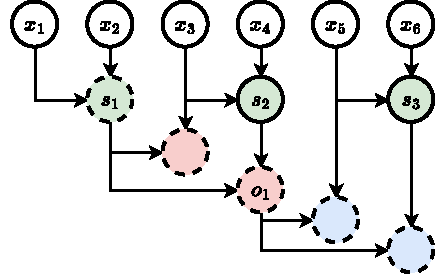
\includegraphics[width=0.45\textwidth]{images/associative_scan}
    \caption{Параллельное сканирование на последовательности из шести элементов: круги одного цвета можно вычислять параллельно; пунктирные круги — это выходы параллельного сканирования.}
    \label{fig:associative_scan}
\end{SCfigure}

В качестве простого примера рассмотрим последовательность из 6 элементов $x_1,x_2,x_3, x_4, x_5, x_6$ (подробный пример, примененный к SSM, можно найти в \cite{smith2022simplified}). Мы будем обозначать через $\hat{x}_i$ $i$-й префикс, который мы хотим вычислить. Общая процедура схематически показана на Рисунке \ref{fig:associative_scan}. Сначала мы агрегируем пары соседних значений как:
%
\begin{align*}
s_1 = x_1 \star x_2  & \rightarrow\hat{x}_2 \\s_2 = x_3 \star x_4 &\\ s_3 = x_5 \star x_6 &
\end{align*}
%
где мы используем стрелки для обозначения выходных значений алгоритма. Теперь мы выполняем второй уровень агрегаций:
%
\begin{align*}
s_1 \star x_3 & \rightarrow \hat{x}_3 \\o_1 = s_1 \star s_2 & \rightarrow \hat{x}_4
\end{align*}
%
И наконец:
%
\begin{align*} 
oalign{
}
oalign{
}o_1 \star x_5 & \rightarrow \hat{x}_5 \\ o_1 \star s_3 & \rightarrow \hat{x}_6
\end{align*}
%
Хотя это выглядит странно (мы сделали 7 шагов вместо 5), три блока вычислений можно тривиально распараллелить, если у нас есть доступ к 3 отдельным потокам. В общем, организуя набор вычислений сбалансированным образом, мы можем вычислить параллельное сканирование за $\mathcal{O}(T \log n)$, где $T$ — стоимость бинарного оператора $\star$. Примером реализации является функция ассоциативного сканирования в JAX.\footnote{\url{https://jax.readthedocs.io/en/latest/_autosummary/jax.lax.associative_scan.html}}

Легко показать, что функция перехода в линейном SSM является примером задачи все-префиксных-сумм. Мы определяем элементы нашей последовательности как пары $x_i = (\mathbf{A}, \mathbf{B}\mathbf{x}_i)$, а бинарный оператор как:
%
$$
(\mathbf{Z}, \mathbf{z})\star (\mathbf{V}, \mathbf{v})=(\mathbf{V}\mathbf{Z}, \mathbf{V}\mathbf{z}+\mathbf{v})
$$
%
Префиксы $\star$ тогда задаются как \cite{smith2022simplified}:
%
$$
x_1 \star x_2 \star \ldots \star x_i=(\mathbf{A}^i, \mathbf{s}_i)
$$
%
Следовательно, запуск параллельного сканирования дает нам степени $\mathbf{A}$ в качестве первых элементов выхода и все состояния слоя в качестве второго элемента выхода. Сложность этой операции ограничена сверху сложностью $\mathbf{A}^{i-1}\mathbf{A}$, которая масштабируется как $\mathcal{O}(n^3)$. Чтобы сделать всю процедуру жизнеспособной, мы можем ограничить $\mathbf{A}$ так, чтобы ее степени можно было вычислять более эффективно. Это тема следующего раздела.

\subsection{Диагональные SSM}

Распространенной стратегией, чтобы сделать предыдущие идеи осуществимыми, является работа с диагональными матрицами перехода (или диагональными матрицами плюс низкоранговый член \cite{gu2021efficiently}). В этом случае степени $\mathbf{A}$ можно легко вычислить, взяв степени диагональных элементов за линейное время. Кроме того, как мы увидим, работа с диагональными матрицами позволяет нам контролировать динамику функции перехода, чтобы избежать численной нестабильности.

В частности, квадратная матрица $\mathbf{A}$ называется \textbf{диагонализируемой}, если мы можем найти другую квадратную (обратимую) матрицу $\mathbf{P}$ и диагональную матрицу $\mathbf{\Lambda}$, такие что:
%$
\begin{equation}
\mathbf{A} = \mathbf{P}\mathbf{\Lambda}\mathbf{P}^{-1}
\label{eq:diagonalizable_A}
\end{equation}
%
Диагонализируемые матрицы (в некотором смысле) «проще», чем общие матрицы. Например, если такое разложение существует, легко показать, что степени также можно эффективно вычислить как:
%
$$
\mathbf{A}^i =\mathbf{P}\mathbf{\Lambda}^i\mathbf{P}^{-1}
$$
%
Предположим, что матрица перехода диагонализируема. Тогда мы можем переписать SSM в эквивалентной форме, имеющей диагональную матрицу перехода. Мы начнем с подстановки \eqref{eq:diagonalizable_A} в определение SSM и умножения с обеих сторон на $\mathbf{P}^{-1}$:
%
$$
\eqnmarkbox[drawred]{node}{\mathbf{P}^{-1}\mathbf{s}_i} =\sum_{j=1}^i\mathbf{\Lambda}^{i-j}\eqnmarkbox[drawgreen]{node2}{\mathbf{P}\mathbf{B}}\mathbf{x}_j
$$
\annotate[yshift=-1em]{below,left}{node}{Новый вектор состояния $\bar{\mathbf{s}}_i$}
\annotate[yshift=-1em]{below,right}{node2}{Новая матрица вход-состояние $\bar{\mathbf{B}}$}

Теперь мы перепишем функцию считывания в терминах новой переменной $\bar{\mathbf{s}}$:
%
$$
\mathbf{y}_i = \eqnmarkbox[drawred]{node}{\mathbf{C}\mathbf{P}}\bar{\mathbf{s}}_i + \mathbf{D}\mathbf{x}_i
$$
\annotate[yshift=-1em]{below,right}{node}{Новая матрица считывания $\bar{\mathbf{C}}$}

\vspace{-0.5em}
Putting everything together:
%
\begin{gather}
\bar{\mathbf{s}}_i=\mathbf{\Lambda}\bar{\mathbf{s}}_{i-1}+\bar{\mathbf{B}}\mathbf{x}_i \\ \mathbf{y}_i=\bar{\mathbf{C}}\bar{\mathbf{s}}_i+ \mathbf{D}\mathbf{x}_i
\end{gather}
%
Следовательно, всякий раз, когда существует диагонализация $\mathbf{A}$, мы всегда можем переписать SSM в эквивалентной форме, имеющей диагональную матрицу перехода. В этом случае мы можем напрямую обучать четыре матрицы $\mathbf{\Lambda} = \text{diag}(\lambda), \lambda \sim (e)$, $\bar{\mathbf{B}} \sim (e,c)$, $\bar{\mathbf{C}} \sim (o,e)$ и $\mathbf{D} \sim (o,c)$, причем диагональная матрица параметризуется одним вектором размерности $e$.

Не все матрицы можно диагонализировать. Однако приближенную диагонализацию всегда можно найти, если разрешить матрицам $\mathbf{P}$ и $\mathbf{\Lambda}$ иметь комплекснозначные элементы \cite{orvieto2023resurrecting}. Необходимо соблюдать осторожность при параметризации значений на диагонали, чтобы собственные значения матрицы перехода оставались $< 1$ по абсолютному значению, чтобы избежать расходящейся динамики. Мы отсылаем к \cite{orvieto2023resurrecting} для описания обоих моментов и для полного анализа результирующего слоя LRU.

\vspace{-1em}
\section{Дополнительные варианты}
%
Балансировка различных сильных сторон свёрток, рекурренции и внимания является активной областью исследований. В заключение книги мы перечислим несколько рекуррентных слоев (или слоев, которые можно интерпретировать как рекуррентные), которые были введены в литературе совсем недавно.
%
\subsection{Трансформеры без внимания}
%
Одна из проблем линеаризованной модели трансформера (Раздел \ref{sec:linearized_transformer_model}) — это квадратичная сложность по размерности признаков $e$. Трансформер без внимания (ATF) был введен как вариант базового слоя внимания, который вместо этого является линейным как по длине последовательности, так и по количеству признаков \cite{zhai2021attention}.

Основная идея заключается в замене взаимодействий скалярного произведения между ключами, запросом и значениями более простым \textit{мультипликативным взаимодействием} (поэлементным):
%
\begin{equation}
\mathbf{h}_i=\sigma(\mathbf{q}_i) \odot\frac{\sum_j \exp\left(\mathbf{k}_j \right) \odot \mathbf{v}_j}{\sum_j\exp\left(\mathbf{k}_j \right)}
\label{eq:atf_new}
\end{equation}
%
Это похоже на слой самовнимания, за исключением того, что мы заменяем все скалярные произведения поэлементными (Адамара) умножениями. Это также вдохновлено линеаризованным слоем внимания в том, что запрос используется только как глобальный модулирующий фактор, в данном случае после его нормализации с помощью операции сигмоида. Фактически, мы можем восстановить стандартную формулировку внимания, переписав \eqref{eq:atf_new} для одной размерности $z$ (используя тот факт, что мы выполняем только поэлементные операции):
%
$$
h_{iz}=\frac{\sigma(q_{iz})\sum_{j}\exp(k_{jz})}{\sum_j \exp(k_{jz})}v_{jz}
$$
%
Следовательно, слой ATF можно переинтерпретировать как поканальный вариант внимания, в том смысле, что для каждого канала мы можем переписать его как операцию внимания над элементами последовательности. Чтобы повысить гибкость, \cite{zhai2021attention} также рассмотрели добавление относительных вложений $\mathbf{W} \sim (m, m)$ (где $m$ — максимальная допустимая длина последовательностей):
%
\begin{equation}\mathbf{h}_i=\sigma(\mathbf{q}_i) \odot\frac{\sum_j \exp\left(\mathbf{k}_j +W_{ij}\right) \odot \mathbf{v}_j}{\sum_j\exp\left(\mathbf{k}_j +W_{ij}\right)}\end{equation}

Относительные вложения также можно обучать с помощью низкоранговой факторизации для уменьшения количества параметров. См. \cite{zhai2021attention} для этого и для дополнительных вариантов базового слоя ATF (например, гибридизации его со свёрточными операциями). Мы также можем преобразовать \eqref{eq:atf_new} в причинный (рекуррентный) вариант, правильно ограничив суммирование.

\subsection{Модель Receptance Weighted Key Value (RWKV)}

Модель RWKV \cite{peng2023rwkv} расширяет слой ATF, включая несколько дополнительных архитектурных модификаций. На момент написания это одна из немногих предварительно обученных РНС, сопоставимых с трансформерами в самом большом масштабе, поэтому мы опишем ее более подробно. Во-первых, относительные вложения упрощаются путем рассмотрения одного вектора $\mathbf{w} \sim (e)$, который масштабируется для каждого смещения:
%
$$
w_{ij}=-(i-j)\mathbf{w}
$$
%
Кроме того, эксперименты показали, что наличие отдельного смещения $\mathbf{u}$ (вместо $\mathbf{w})$ для текущего элемента полезно. Записанное в причинной форме, это дает:

\begin{equation}
\mathbf{h}_i={\color{drawred}\mathbf{W}_o\Biggl(\Bigr.}\sigma(\mathbf{q}_i) \odot\frac{{\color{drawred}\sum_{j=1}^{i-1}}\exp\left(\mathbf{k}_j +w_{ij}\right) \odot \mathbf{v}_j{\color{drawred}+\exp\left(\mathbf{k}_i+\mathbf{u}\right) \odot \mathbf{v}_i}}{{\color{drawred}\sum_{j=1}^{i-1}}\exp\left(\mathbf{k}_j +w_{ij}\right){\color{drawred}+\exp\left(\mathbf{k}_i+\mathbf{u}\right)}}{\color{drawred}\Bigl.\Biggr)}
\label{eq:rwkv}
\end{equation}

где мы выделяем красным цветом отличия от базового слоя ATF. Запрос называется \textbf{рецептансом} в \cite{peng2023rwkv}, и в конце добавляется дополнительная выходная проекция $\mathbf{W}_o$. Во-вторых, модель RWKV изменяет стандартный МЛП в блоке трансформера на по-другому \textit{вентильный} токен-ориентированный блок. Для данного входного токена $\mathbf{x}$ это можно записать как:
%
\begin{equation}\mathbf{y}=\sigma(\mathbf{W}_1\mathbf{x})\odot \mathbf{W}_2\max(0, \mathbf{W}_3\mathbf{x})^2\end{equation}

где $\mathbf{W}_1$, $\mathbf{W}_2$ и $\mathbf{W}_3$ — обучаемые параметры. Это стандартный МЛП, за исключением левого вентиля и использования квадрата ReLU. В качестве последней модификации все три проекции в первом блоке (а также два появления $\mathbf{x}$ в \eqref{eq:rwkv}) заменяются выпуклыми комбинациями $\mathbf{x}_i$ и $\mathbf{x}_{i-1}$ для улучшения производительности, что называется \textit{сдвигом токенов}.

\subsection{Селективные модели в пространстве состояний}

Мы рассмотрели три класса рекуррентных моделей: стандартные рекуррентные слои (и их вентильные версии), линеаризованные слои внимания и структурированные модели в пространстве состояний. Хотя они выглядят по-разному, относительно легко перейти от одного класса моделей к другому. Чтобы убедиться в этом, давайте рассмотрим линеаризованный слой внимания, где мы игнорируем знаменатель:
%
\begin{align}
\mathbf{S}_i=\mathbf{S}_{i-1}+\phi(\mathbf{k}_i)\mathbf{v}_i^\top \label{eq:lin_att_simplified_1} \\
\mathbf{h}_i=\phi(\mathbf{q}_i)^\top\mathbf{S}_i
\label{eq:lin_att_simplified_2}\end{align}
%
Помимо матричнозначного состояния, мы видим, что это имеет форму слоя SSM, за исключением того, что некоторые матрицы (например, $\mathbf{C} = \phi(\mathbf{q}_i)^\top$) не фиксированы, а зависят от конкретного входного токена. С точки зрения динамических систем, мы говорим, что стандартные SSM описывают \textit{инвариантные во времени} системы, в то время как \eqref{eq:lin_att_simplified_1}-\eqref{eq:lin_att_simplified_2} описывают \textit{изменяющуюся во времени} систему. Это вдохновило другой класс слоев SSM, чьи матрицы не ограничены быть инвариантными во времени, которые были названы \textbf{селективными} SSM. Большинство этих моделей используют идею слоев внимания о многократном проецировании входа перед вычислениями слоя.

\begin{SCfigure}
    \centering
    \hspace{2em}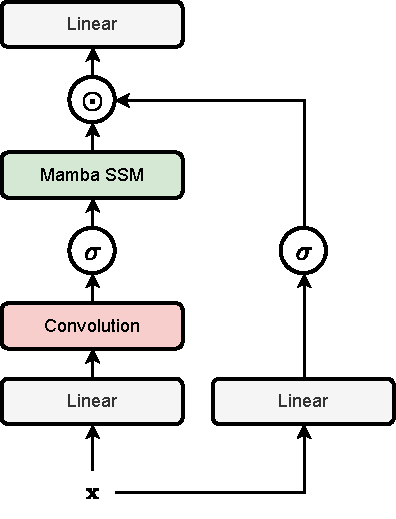
\includegraphics[width=0.4\textwidth]{images/mamba}
    \caption{Блок Mamba (остаточные соединения вокруг блока и нормализация не показаны). $\sigma$ — это функция сигмоида. Адаптировано из \cite{gu2023mamba}.}
    \label{fig:mamba}
\end{SCfigure}

В качестве примера мы сосредоточимся здесь на так называемом слое Mamba \cite{gu2023mamba}, который на момент написания является одним из немногих слоев SSM, который был масштабирован до соответствия производительности моделей-трансформеров при очень больших контекстах и количестве параметров. Во-первых, чтобы сделать слой SSM изменяющимся во времени, подмножество его матриц делается зависимым от входа:\footnote{Матрица $\mathbf{D}$ может рассматриваться как простое остаточное соединение и остается неизменной. Оригинальный слой имеет немного другую параметризацию, где $\mathbf{A} = \exp(\Delta \bar{\mathbf{A}})$, для некоторого обучаемого $\bar{\mathbf{A}}$ и зависящего от входа скалярного значения $\Delta$. Это не меняет нашего обсуждения.}
%
\begin{gather}
\mathbf{s}_i = A(\mathbf{x}_i)\mathbf{s}_{i-1} + B(\mathbf{x}_i)\mathbf{x}_i \\ \mathbf{h}_i = C(\mathbf{x}_i)\mathbf{s}_i + \mathbf{D}\mathbf{x}_i 
\end{gather}
%
где $A(\bullet)$, $B(\bullet)$ и $C(\bullet)$ — это линейные проекции их входных токенов. Чтобы сделать это возможным, слой применяется к каждому каналу входа независимо, а матрица перехода выбирается диагональной, так что все матрицы SSM могут быть представлены одним вектором значений. Этот слой теряет простую реализацию параллельного сканирования и требует индивидуальной реализации, учитывающей аппаратное обеспечение \cite{gu2023mamba}. Можно показать, что вариант Mamba SSM и несколько других слоев SSM являются вырожденным случаем вентильного рекуррентного слоя \cite{gu2021combining,gu2023mamba}.

Чтобы сделать общую архитектуру проще, Mamba избегает чередования МЛП и SSM в пользу вентильной архитектуры (похожей на вентильный блок внимания из Раздела \ref{subsec:mha_variants}), где МЛП используется для взвешивания выходов из SSM. Добавляется дополнительная глубинная свёртка для повышения гибкости - см. Рисунок \ref{fig:mamba}.